\section{Cálculo analítico de la fuerza de atracción}
\label{sec:analitico}
En la sección de desarrollo teórico trataré de proporcionar un procedimiento mediante el cual los alumnos que realicen la práctica sean capaces de optimizar la velocidad y fuerza del proyectil a partir de los parámetros eléctricos y geométricos que definen el sistema. Estos parámetros de entrada serán:
\begin{itemize}
    \item \textbf{Parámetros geométricos}:
    \begin{enumerate}[label=\alph*., leftmargin=*, itemindent=1em]
        \item \(r_{cext}\) y \(r_{cint} \): radios exterior e interior de la bobina, respectivamente.
        \item \(l_c\): altura de la bobina.
        \item \(r_{fe}\): radio del vástago.
        \item \(l_{fe}\): longitud del vástago.
        \item \(k_{disp}\): parámetro multiplicador para obtener la sección de dispersión. La dispersión es la parte del flujo que abraza a la bobina y a la barra.
    \end{enumerate}
    \item \textbf{Parámetros electromagnéticos}:
    \begin{enumerate}[label=\alph*., leftmargin=*, itemindent=1em]
        \item \(N\): número de espiras.
        \item \(I_{cc}\): corriente de alimentación del solenoide.
        \item \(\mu_{fe}\): permeabilidad relativa del vástago ferromagnético.
    \end{enumerate}
\end{itemize}

\begin{figure}[H]
    \centering 
    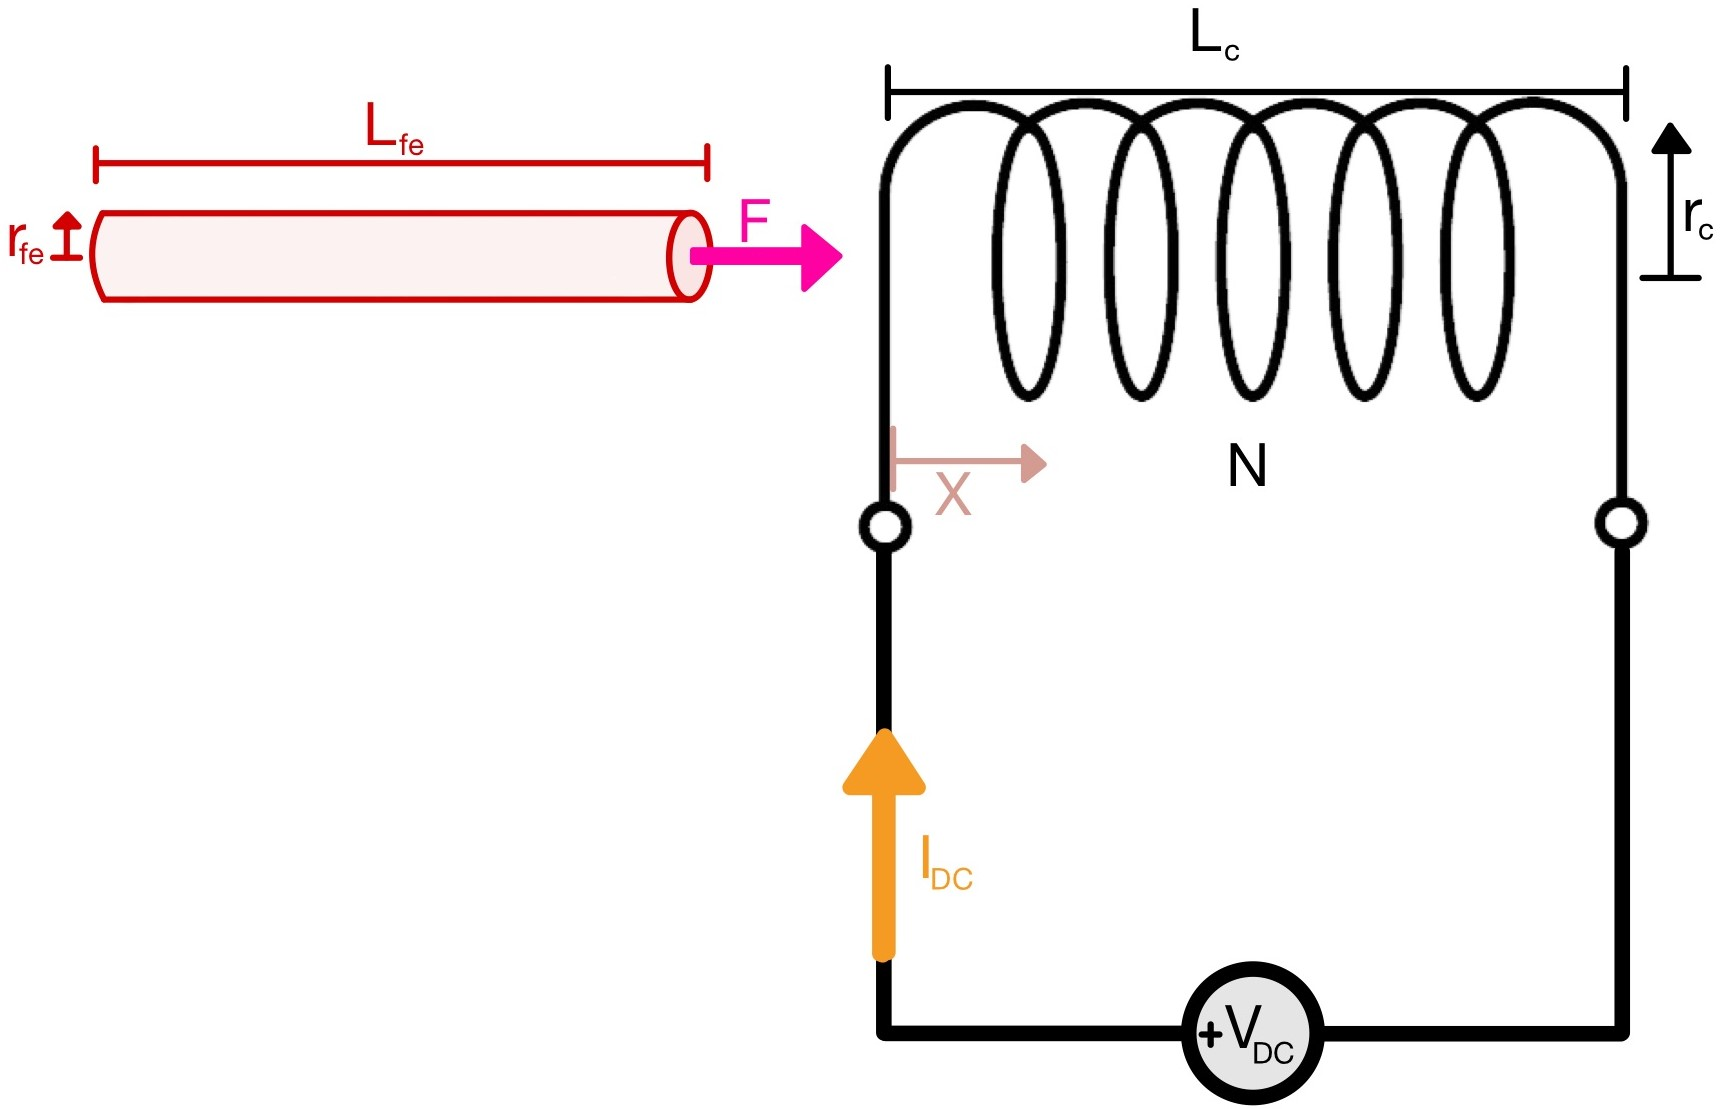
\includegraphics[width=9cm]{FigurasMemoria/esquemaDesTeor.jpg}
    \caption{Esquema geométrico del sistema.}
    \label{fig:esquemaDesTeor} %Para referenciar -> \ref{fig:figNum}
\end{figure}

El objetivo de este desarrollo es crear un programa en MATLAB al que se le proporcionen estos datos, y con ellos calcule automáticamente la fuerza que experimentará el proyectil a través del circuito magnético del sistema. Como se muestra en la figura \ref{fig:electromagnet} el valor de \(B\) varía a lo largo del solenoide, por lo tanto, además de los parámetros constantes dados, será necesario parametrizar también la posición del vástago en cada momento (\(x\) en la figura \ref{fig:esquemaDesTeor}) y calcular la fuerza que experimenta en cada una de esas posiciones.

El primer paso será partir de las fórmulas del circuito magnético definidas en el apartado de marco teórico (\ref{sec:marcoteorico}) y para ello la primera tarea es realizar un análisis de las diferentes reluctancias del sistema, con el objetivo de computar así la inducción magnética, la cual nos permitirá obtener la fuerza de atracción que experimenta el vástago, que según Nicolás Jerez \citep{jerez2016resueltos} viene dada por la expresión:

\begin{center}
\[F=\frac{1}{2}\frac{B^2*S}{\mu_0}\]
\end{center}

Teniendo clara la relación entre inducción y fuerza, el siguiente paso es definir claramente las diferentes áreas efectivas de los componentes del sistema para calcular las reluctancias, las cuales son:

\begin{itemize}
    \item \(S_{c}=\pi *r_{cext}^2\): Esta superficie se corresponde con la sección delimitada por el radio exterior de la bobina, y es el área efectiva del flujo encerrado en su interior.
    \item \(S_{fe}=\pi *r_{fe}^2\): Esta superficie se corresponde con la sección delimitada por el radio del vástago.
    \item \(S_{disp}=\pi *r_{disp}~~\forall r_{disp} = k_{disp}r_c\): Esta superficie se corresponde con el área de dispersión de flujo, la cual se relacionará con una reluctancia no obvia del sistema que modela el (escaso) flujo magnético que se dispersa a través del aire que rodea el sistema.
\end{itemize}

\begin{figure}[H]
    \centering
    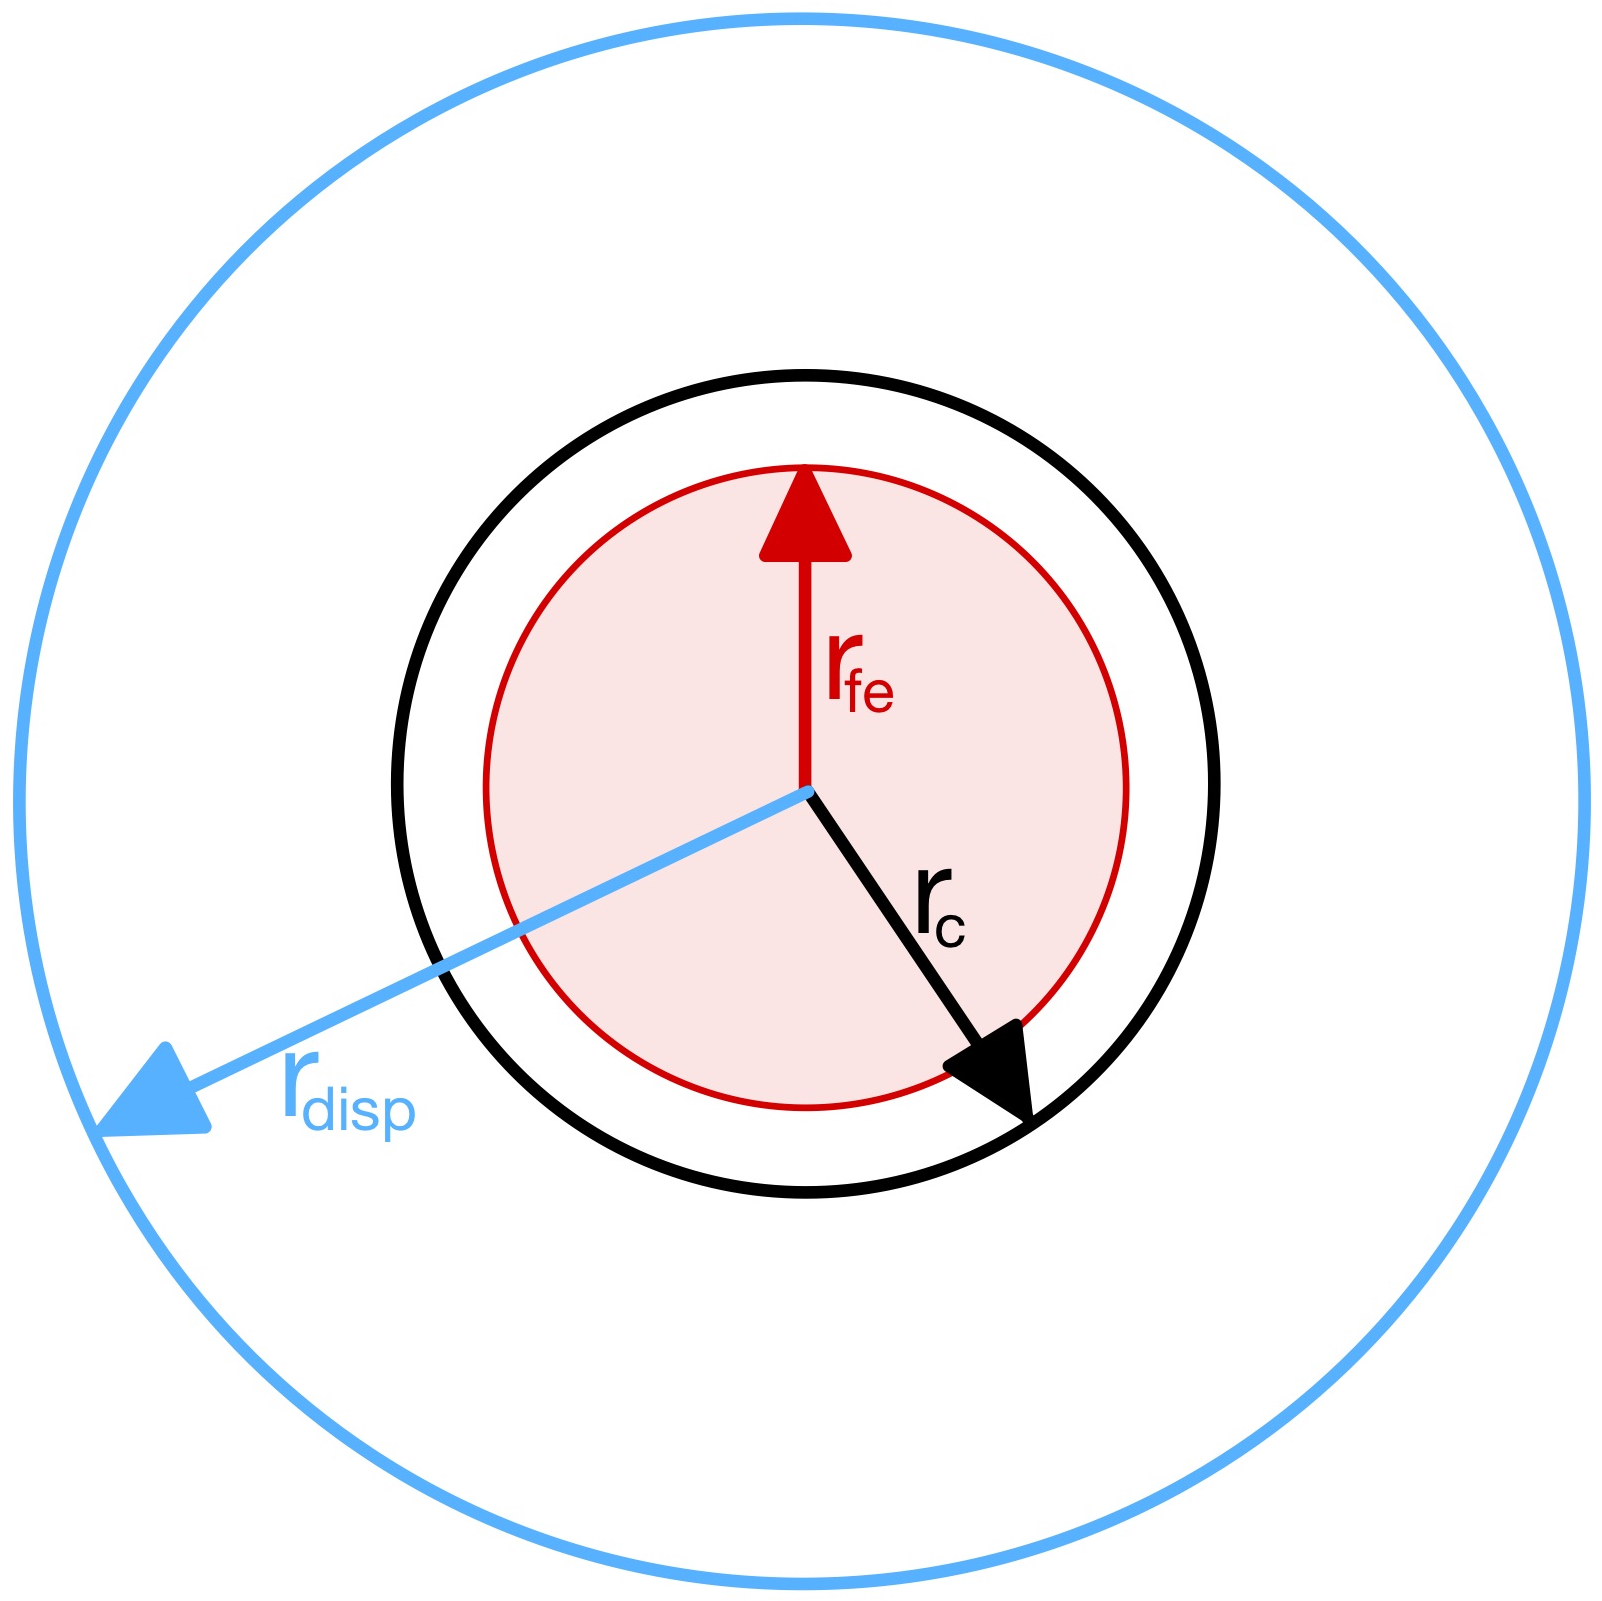
\includegraphics[width=4.5cm]{FigurasMemoria/areasFlujo.jpg}
    \caption{Secciones del sistema con una vista de planta.}
    \label{fig:areasFlujo} %Para referenciar -> \ref{fig:figNum}
\end{figure}

Teniendo en cuenta las fórmulas en la sección del marco teórico (\ref{sec:marcoteorico}) y lo expuesto en la figura \ref{fig:areasFlujo}, podemos concluir que existen cuatro principales reluctancias en el sistema de la figura \ref{fig:esquemaDesTeor}:

\begin{itemize}
    \item \(\mathcal{R}_{disp~c}=\frac{h_c}{\mu_0*S_{disp}}\): Se corresponde a la reluctancia del aire que abraza la bobina. Esta reluctancia es fija ya que las dimensiones del solenoide son constantes.
    \item \(\mathcal{R}_{fe}=\frac{l_{fe}}{\mu_0*\mu_{fe}*S_{fe}}\): Se corresponde a la reluctancia de la barra. Esta reluctancia es fija ya que las dimensiones del vástago son constantes.
    \item \(\mathcal{R}_{\phi}=\frac{(h_c+l_{fe})-x}{\mu_0*S_{disp}}\): Se corresponde a la reluctancia del aire del camino más largo del flujo magnético, y es la que provoca que el campo del electroimán interactúe con el vástago. Es variable ya que la posición del vástago es variable, y el camino se reduce con el tiempo.
    \item \(\mathcal{R}_{aire~c}=\frac{h_c-x}{\mu_0*S_c}\): Se corresponde a la reluctancia del aire en el interior de la bobina. Es variable ya que la cantidad de aire dentro de la misma disminuye según el vástago aumenta.
\end{itemize}

\begin{figure}[H]
    \centering
    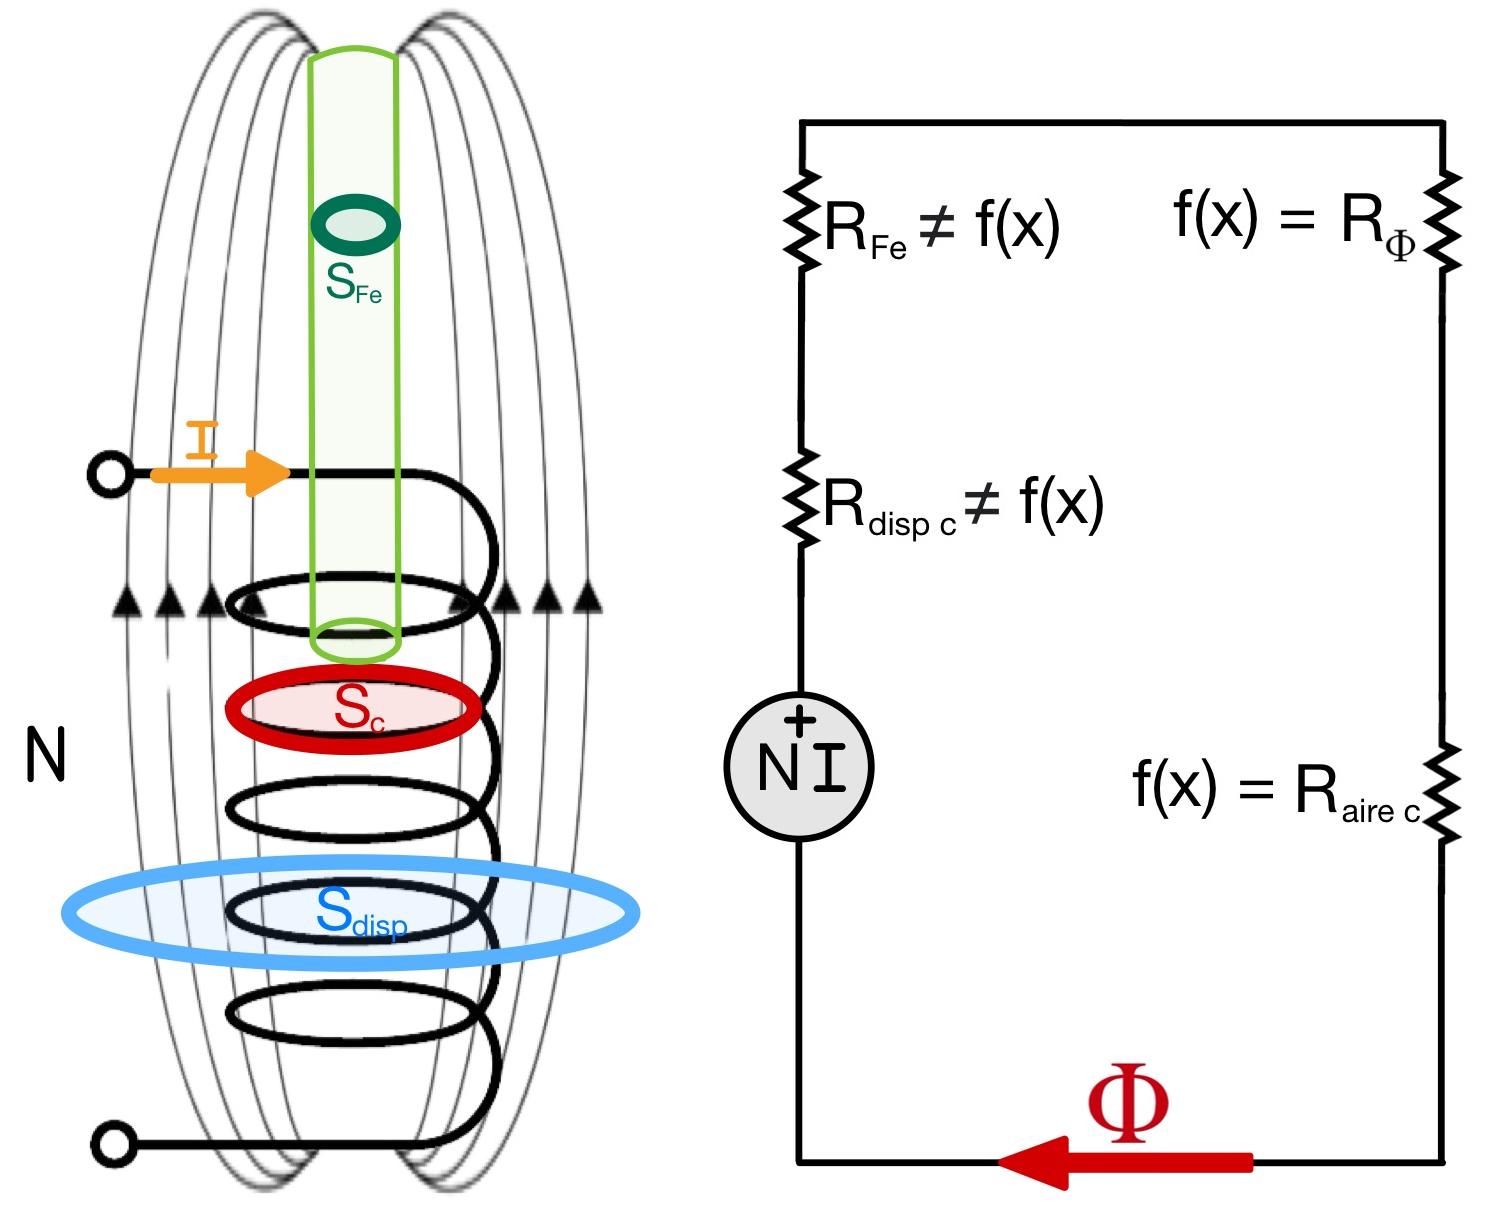
\includegraphics[width=11cm]{FigurasMemoria/circuitoMag.jpg}
    \caption{Circuito magnético del sistema.}
    \label{fig:circuitoMag} %Para referenciar -> \ref{fig:figNum}
\end{figure}


Con el circuito magnético definido, el siguiente paso es programar las relaciones presentadas en esta sección en \textit{MatLAB}\textregistered y graficar los resultados en función de la posición. El programa en \textit{MatLAB}\textregistered constará de tres secciones: definición, cálculos y graficación. El código se puede encontrar en el anexo 1. El producto de este código es una ``calculadora'' que devuelve la evolución de la fuerza con el parámetro \(x\), y queda así:

\begin{figure}[H]
    \centering
    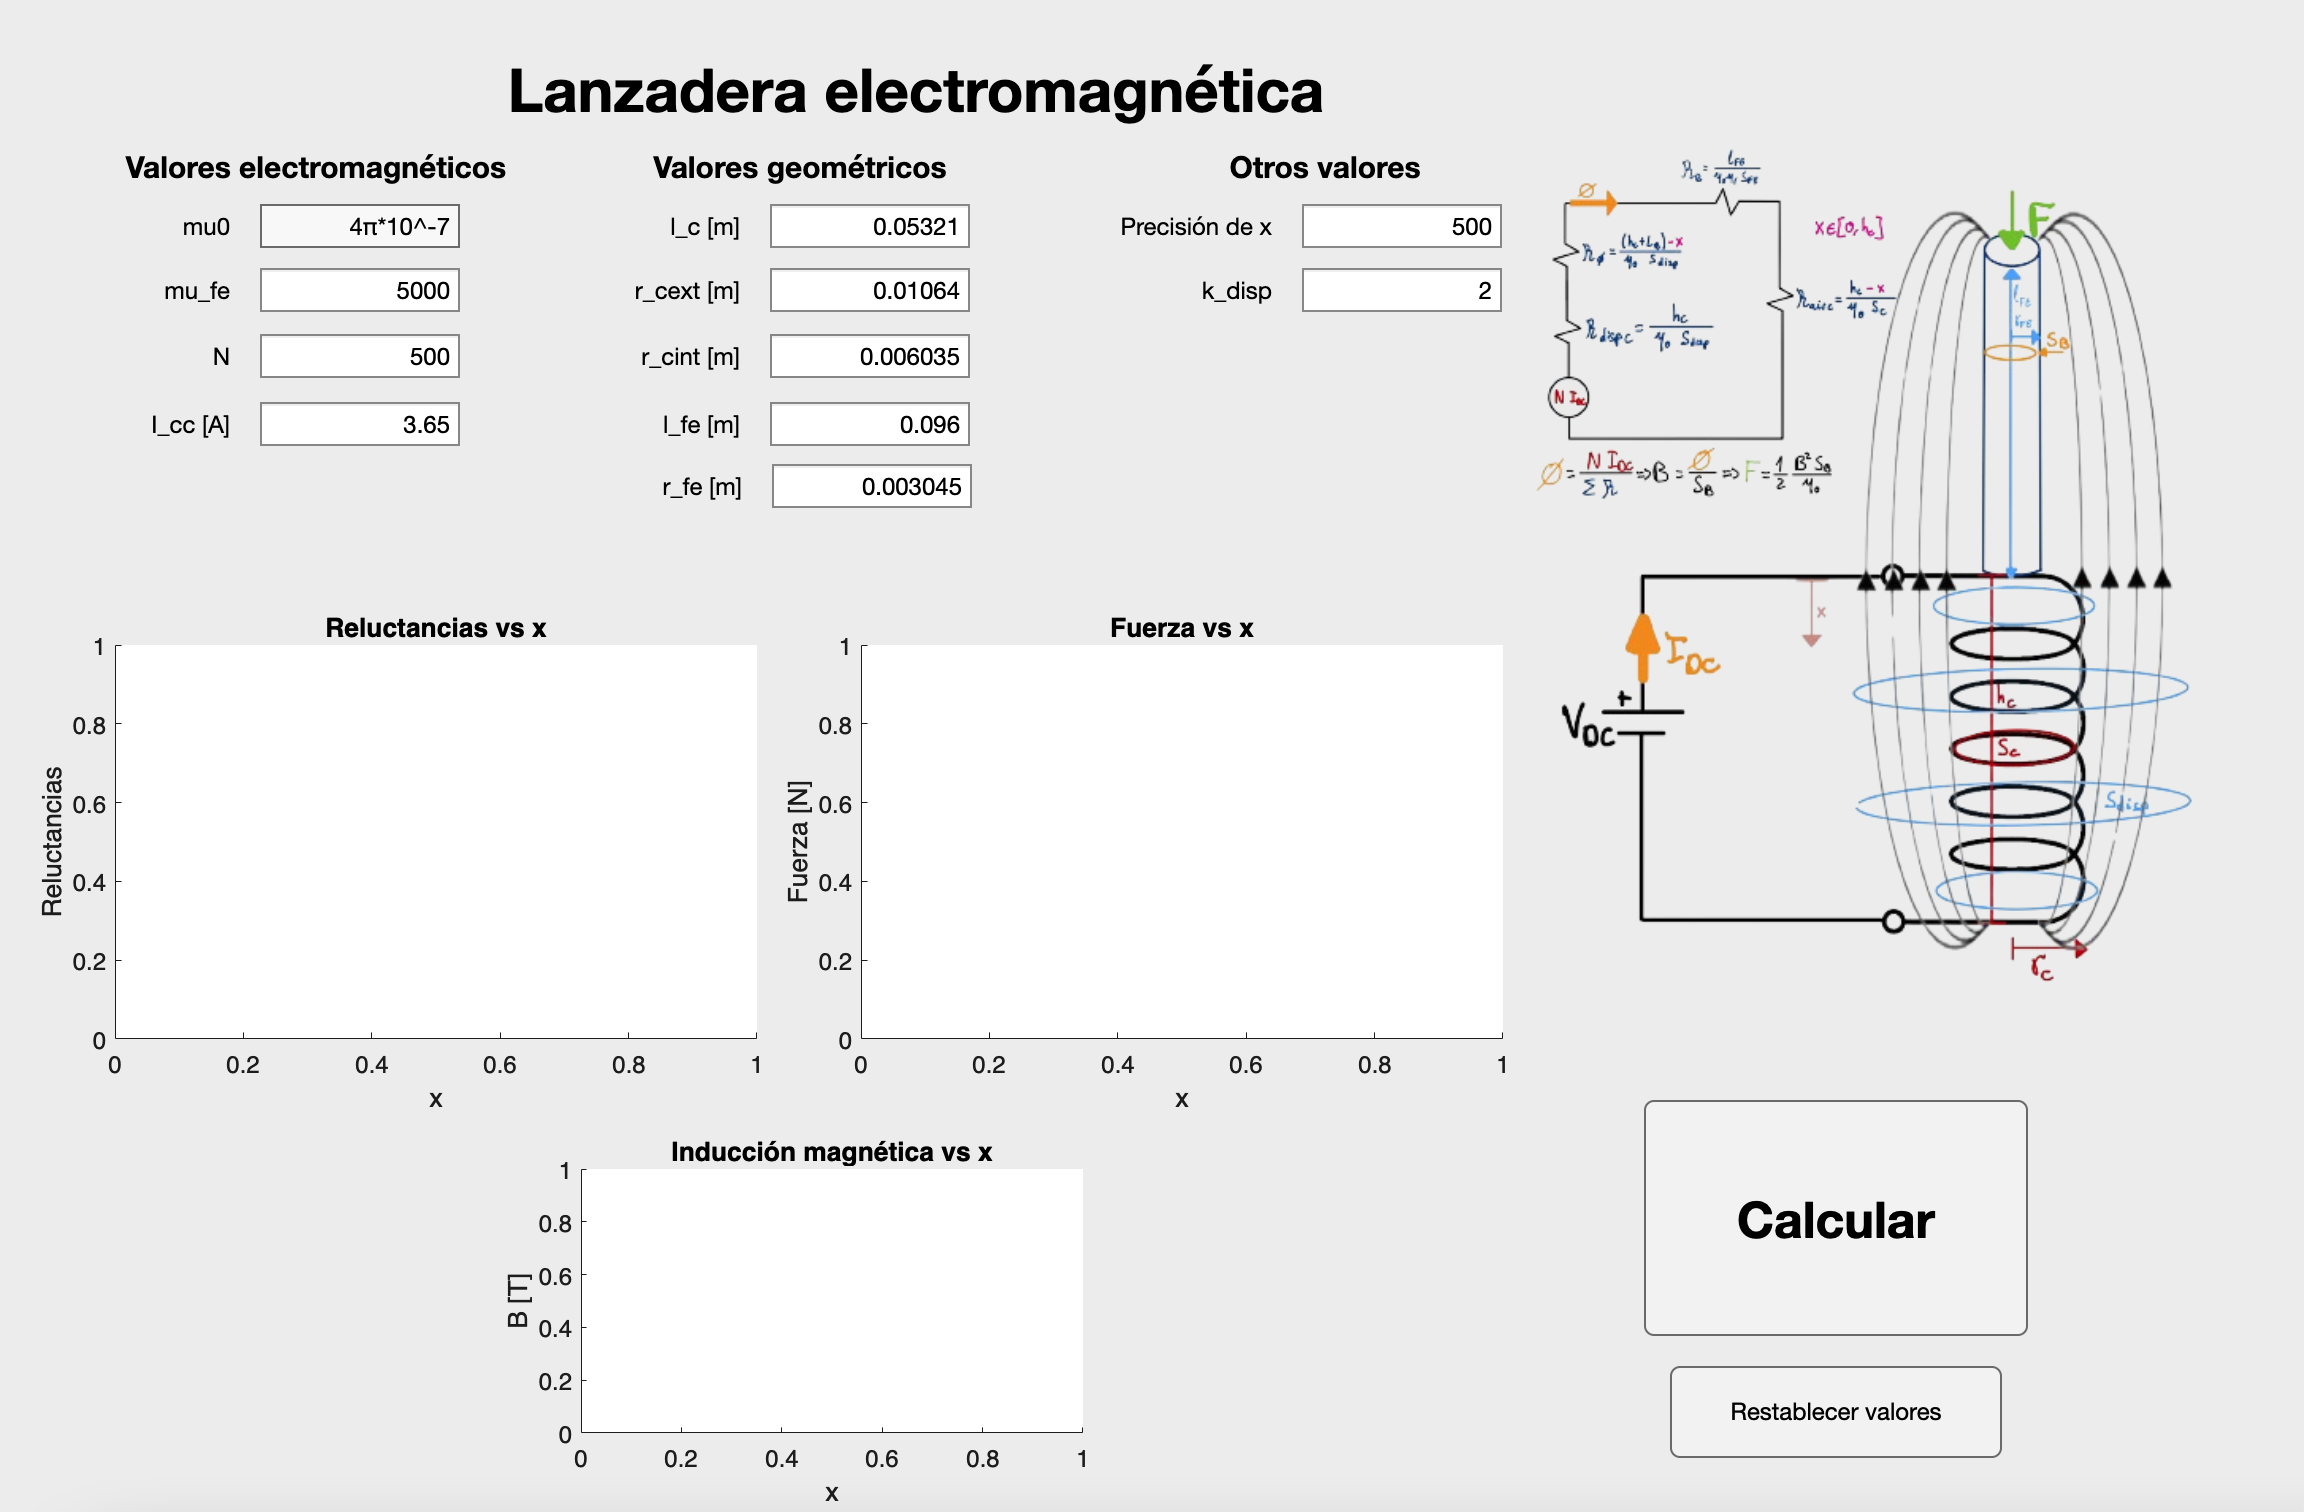
\includegraphics[width=\linewidth]{FigurasMemoria/calculadora.png}
    \caption{Aplicación de cálculos de \textit{MatLAB}\textregistered.}
    \label{fig:calculadora} %Para referenciar -> \ref{fig:figNum}
\end{figure}

\newpage

Los valores escritos en las variables del sistema que se pueden ver en la figura \ref{fig:calculadora} se correponden con la bobina de ejemplo que se ha utilizado para crear el proyecto. Dicha bobina tiene la siguiente geometría:

\[
\begin{array}{c}
    \mu_0 = 4\pi \times 10^{-7}~~~~~~\mu_{fe} = 5000~~~~~~N = 500 ~~~~~~ k_{disp} = 2 \\
    l_{fe} = 0.096m~~~~~~r_{fe} = 0.003045m \\
    l_c = 0.05321m~~~~~~r_{cext} = 0.01064m~~~~~~r_{cint}=0.006035 
\end{array}
\]

Con esta configuración, la forma de las gráficas obtenidas es:

\begin{figure}[H]
    \centering
    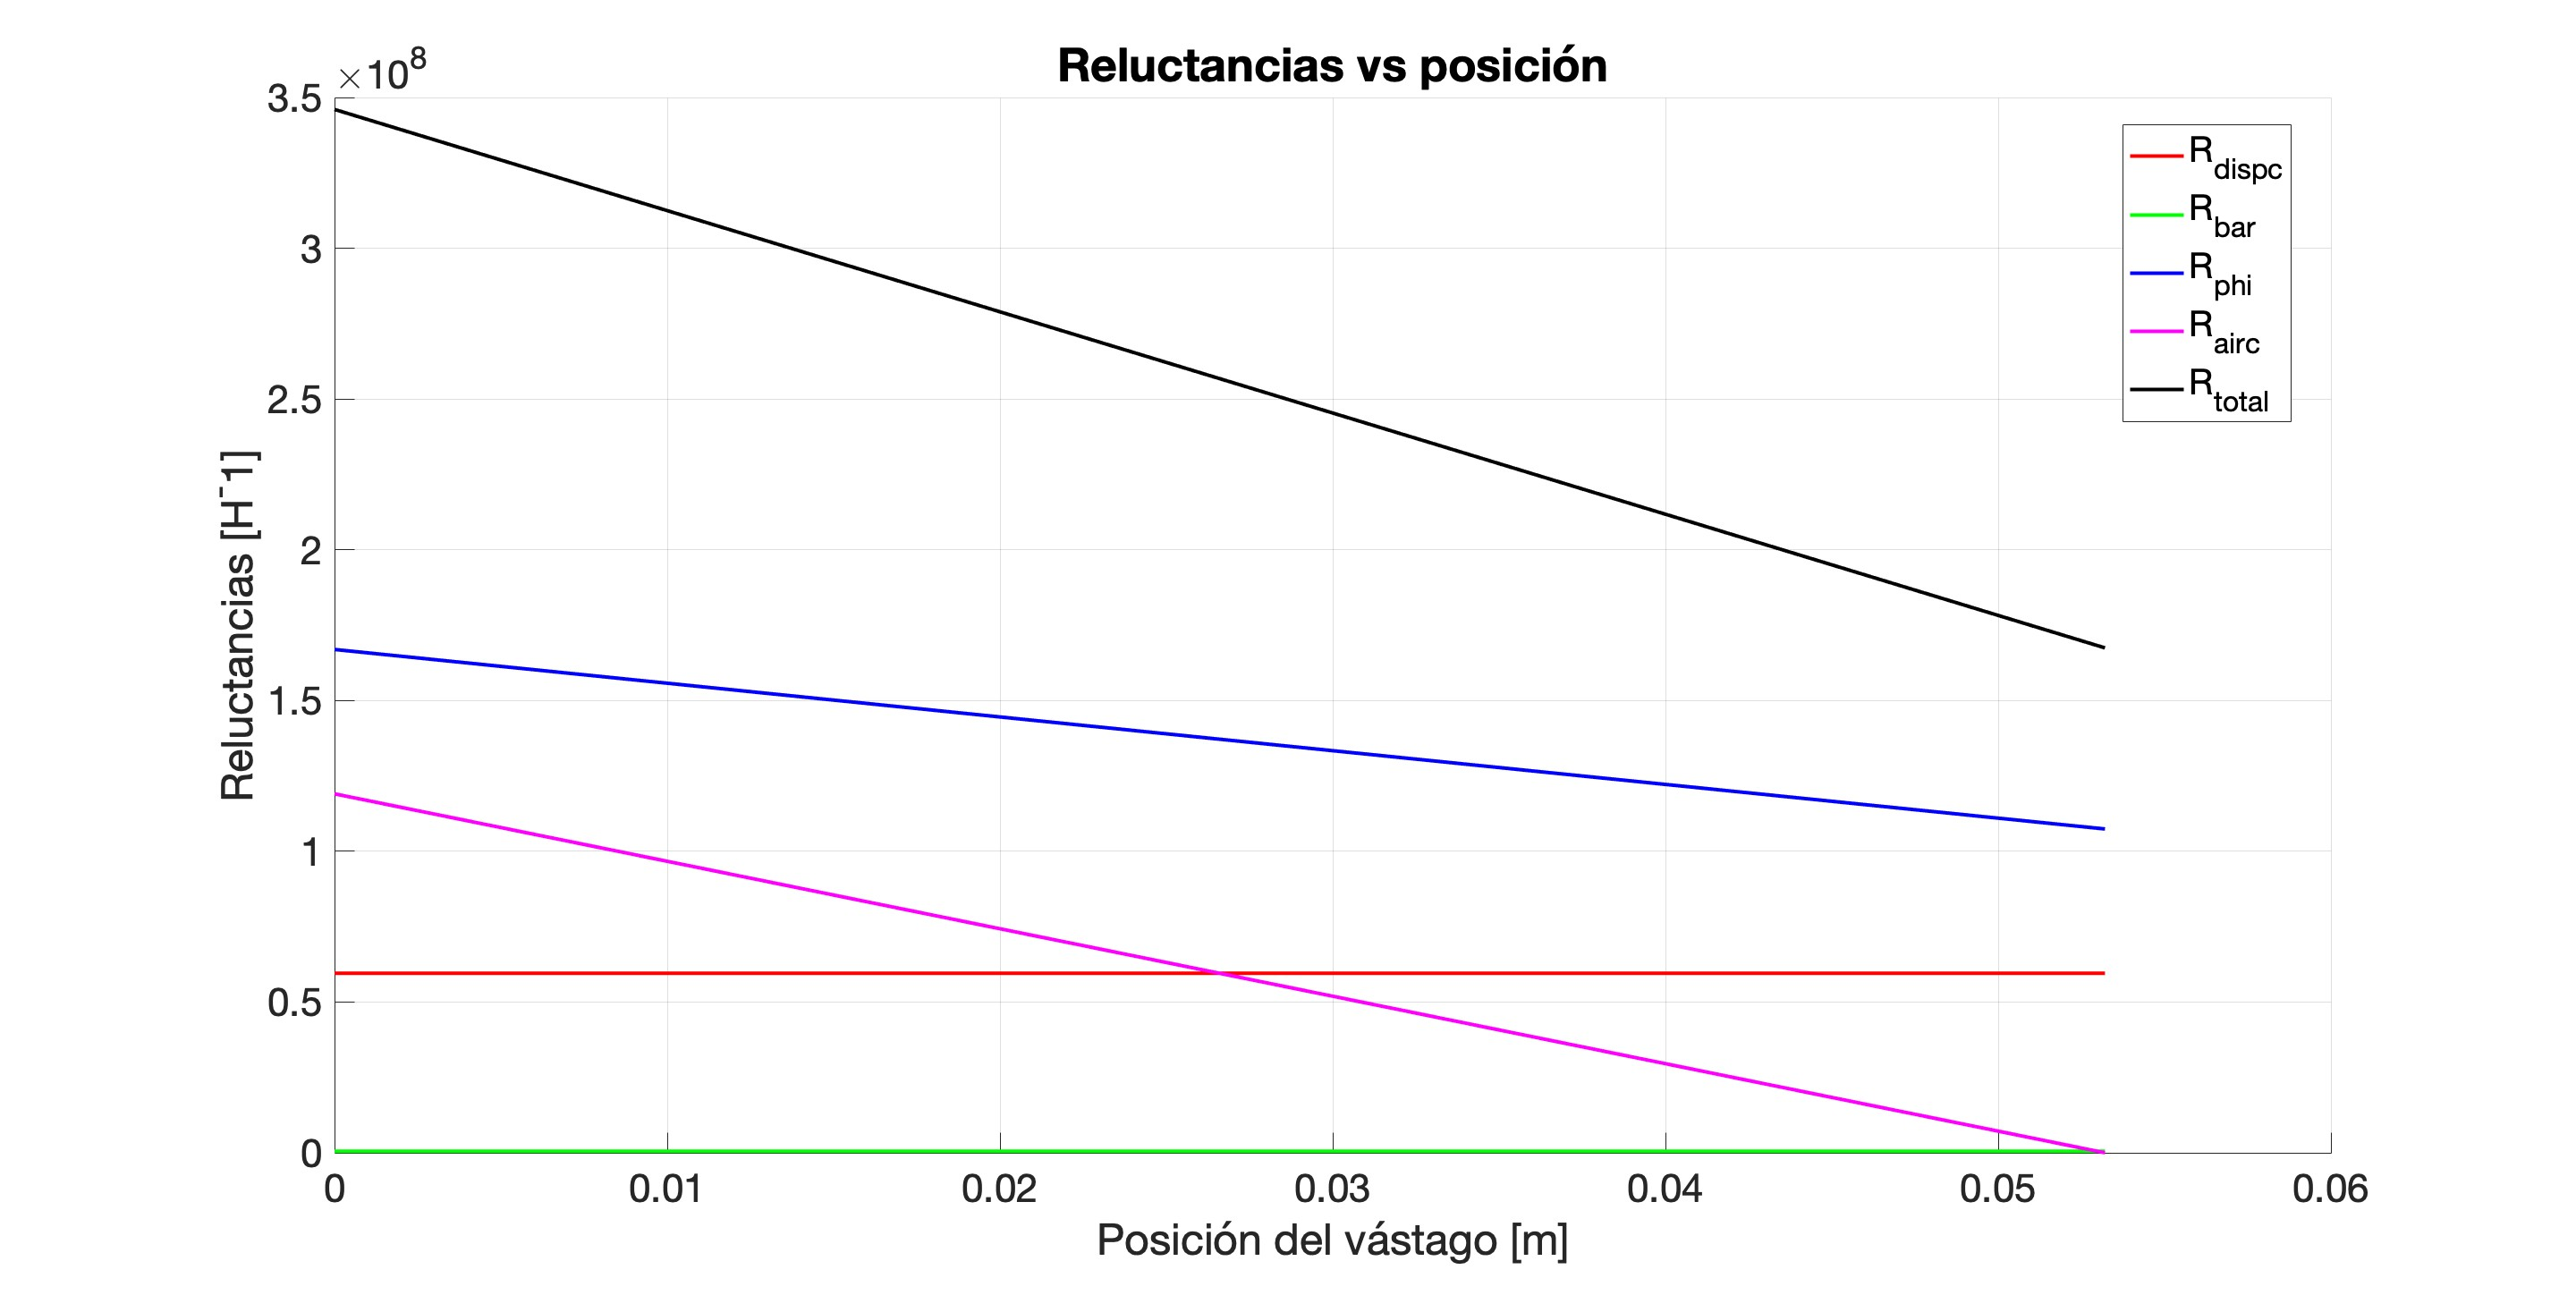
\includegraphics[width=\linewidth]{FigurasMemoria/calcRsetupBase.jpg}
    \caption{Reluctancias en función de la posición del vástago respecto a la bobina.}
    \label{fig:calcRsetupBase} %Para referenciar -> \ref{fig:figNum}
\end{figure}

\begin{figure}[H]
    \centering
    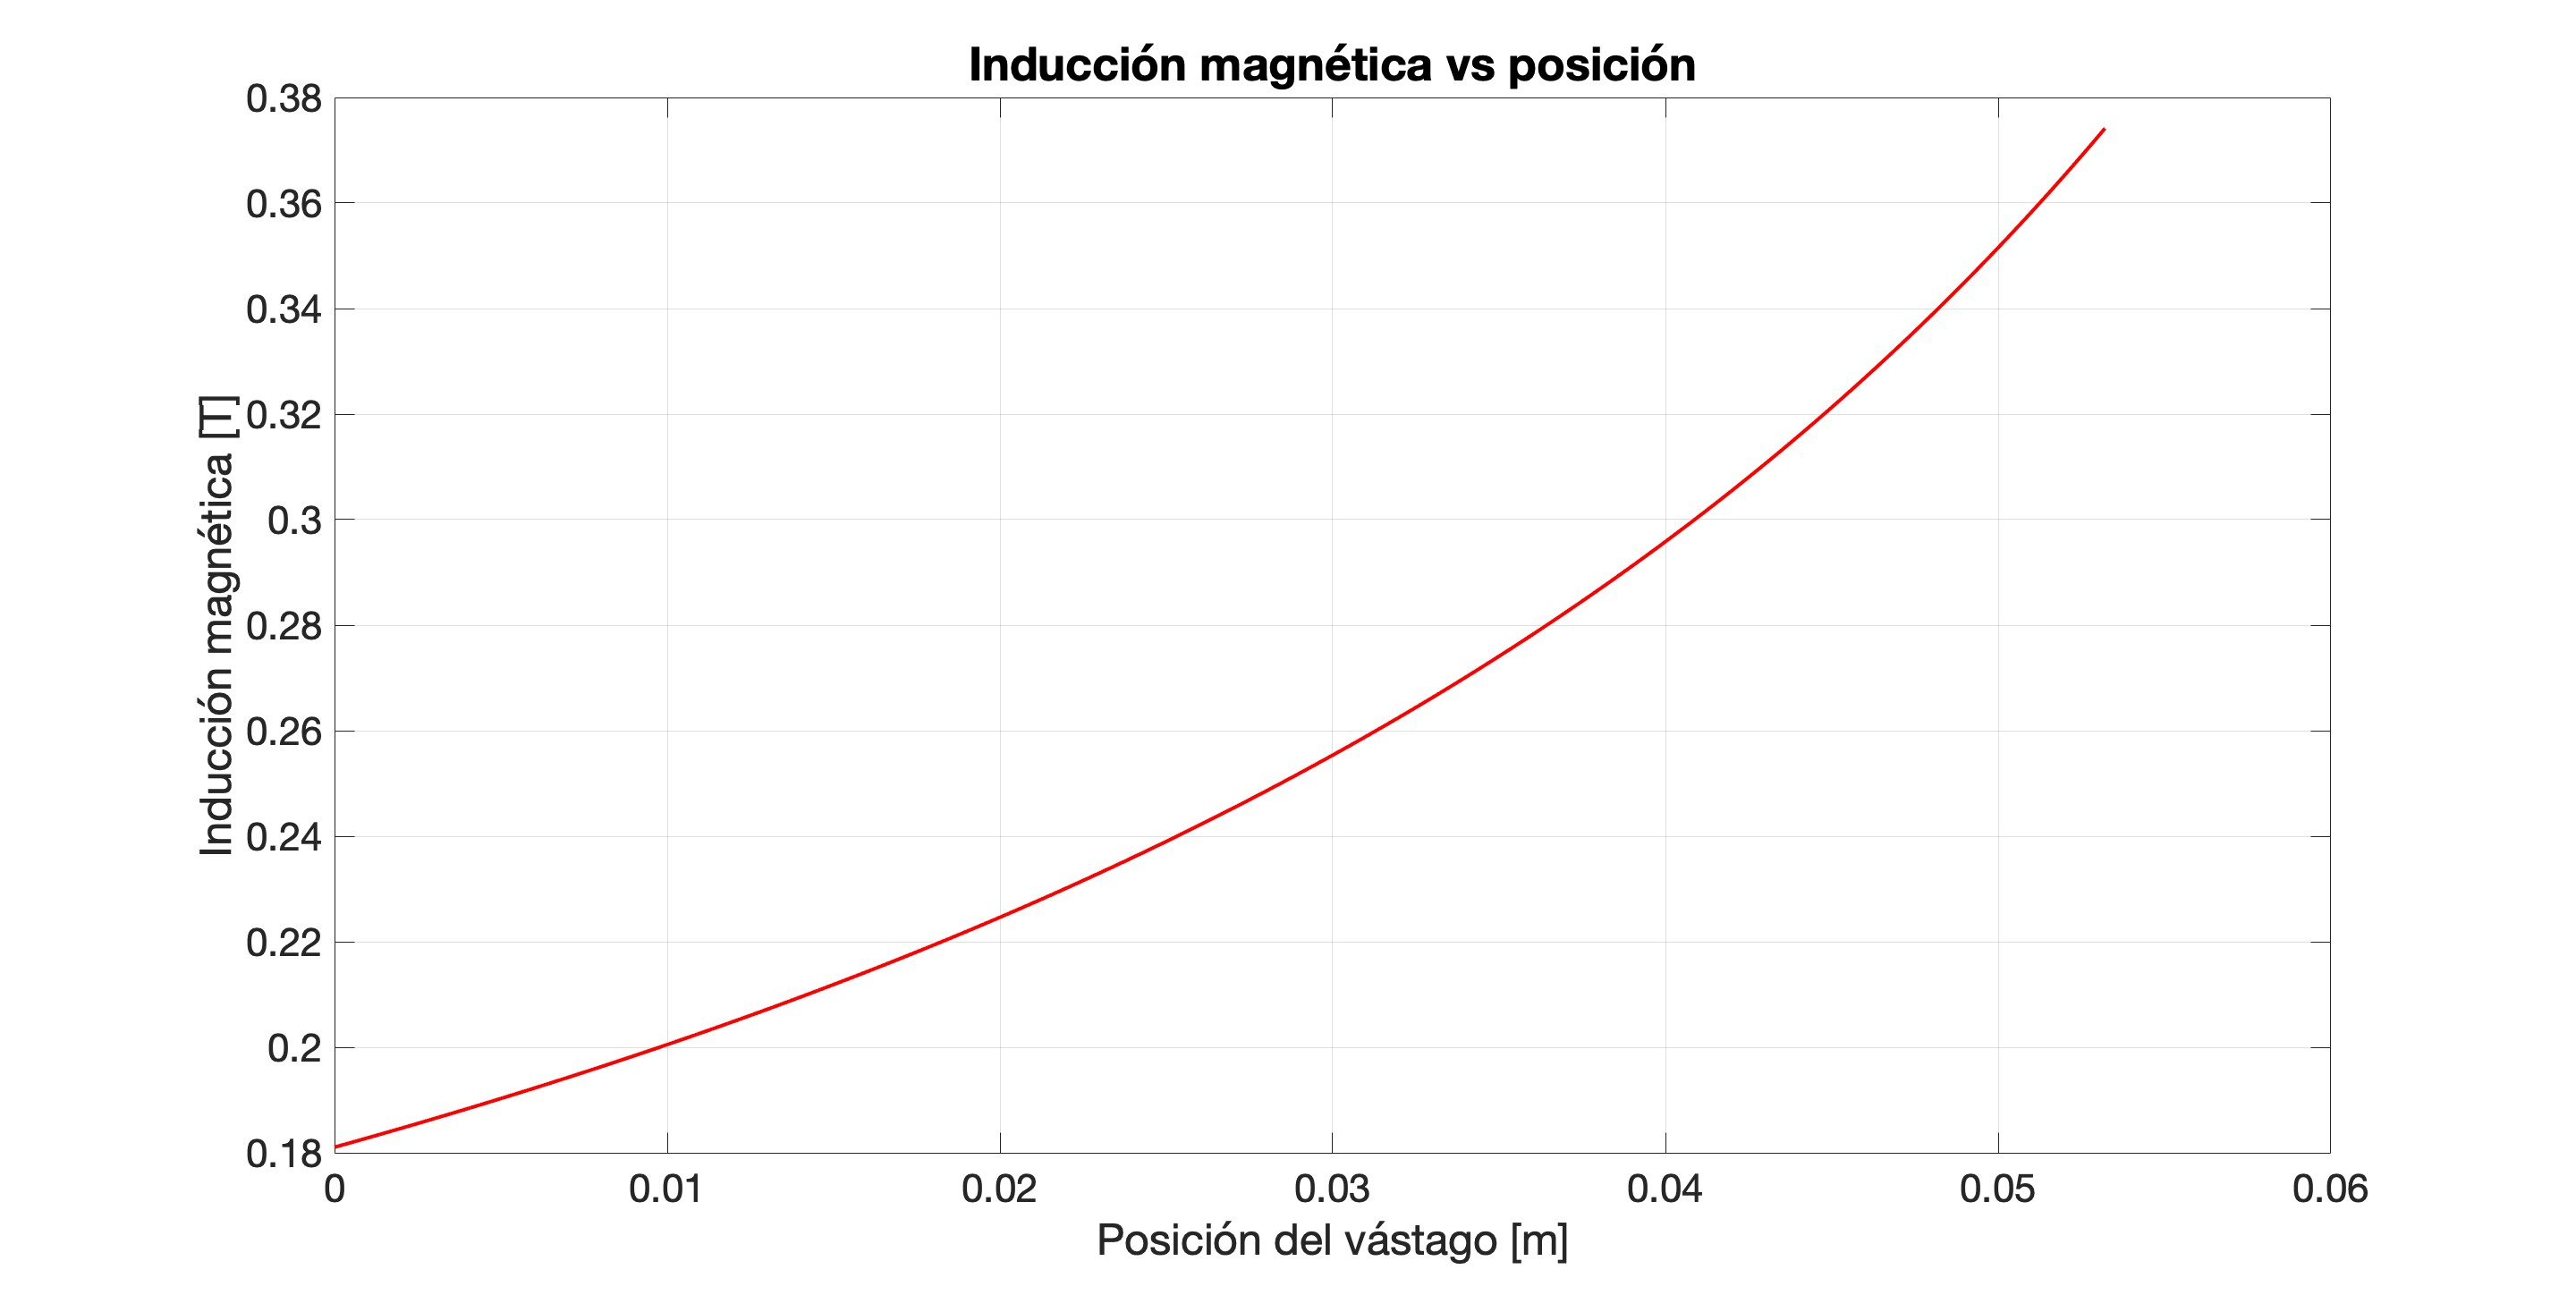
\includegraphics[width=\linewidth]{FigurasMemoria/calcBsetupBase.jpg}
    \caption{Inducción en función de la posición del vástago respecto a la bobina.}
    \label{fig:calcBsetupBase} %Para referenciar -> \ref{fig:figNum}
\end{figure}

\begin{figure}[H]
    \centering
    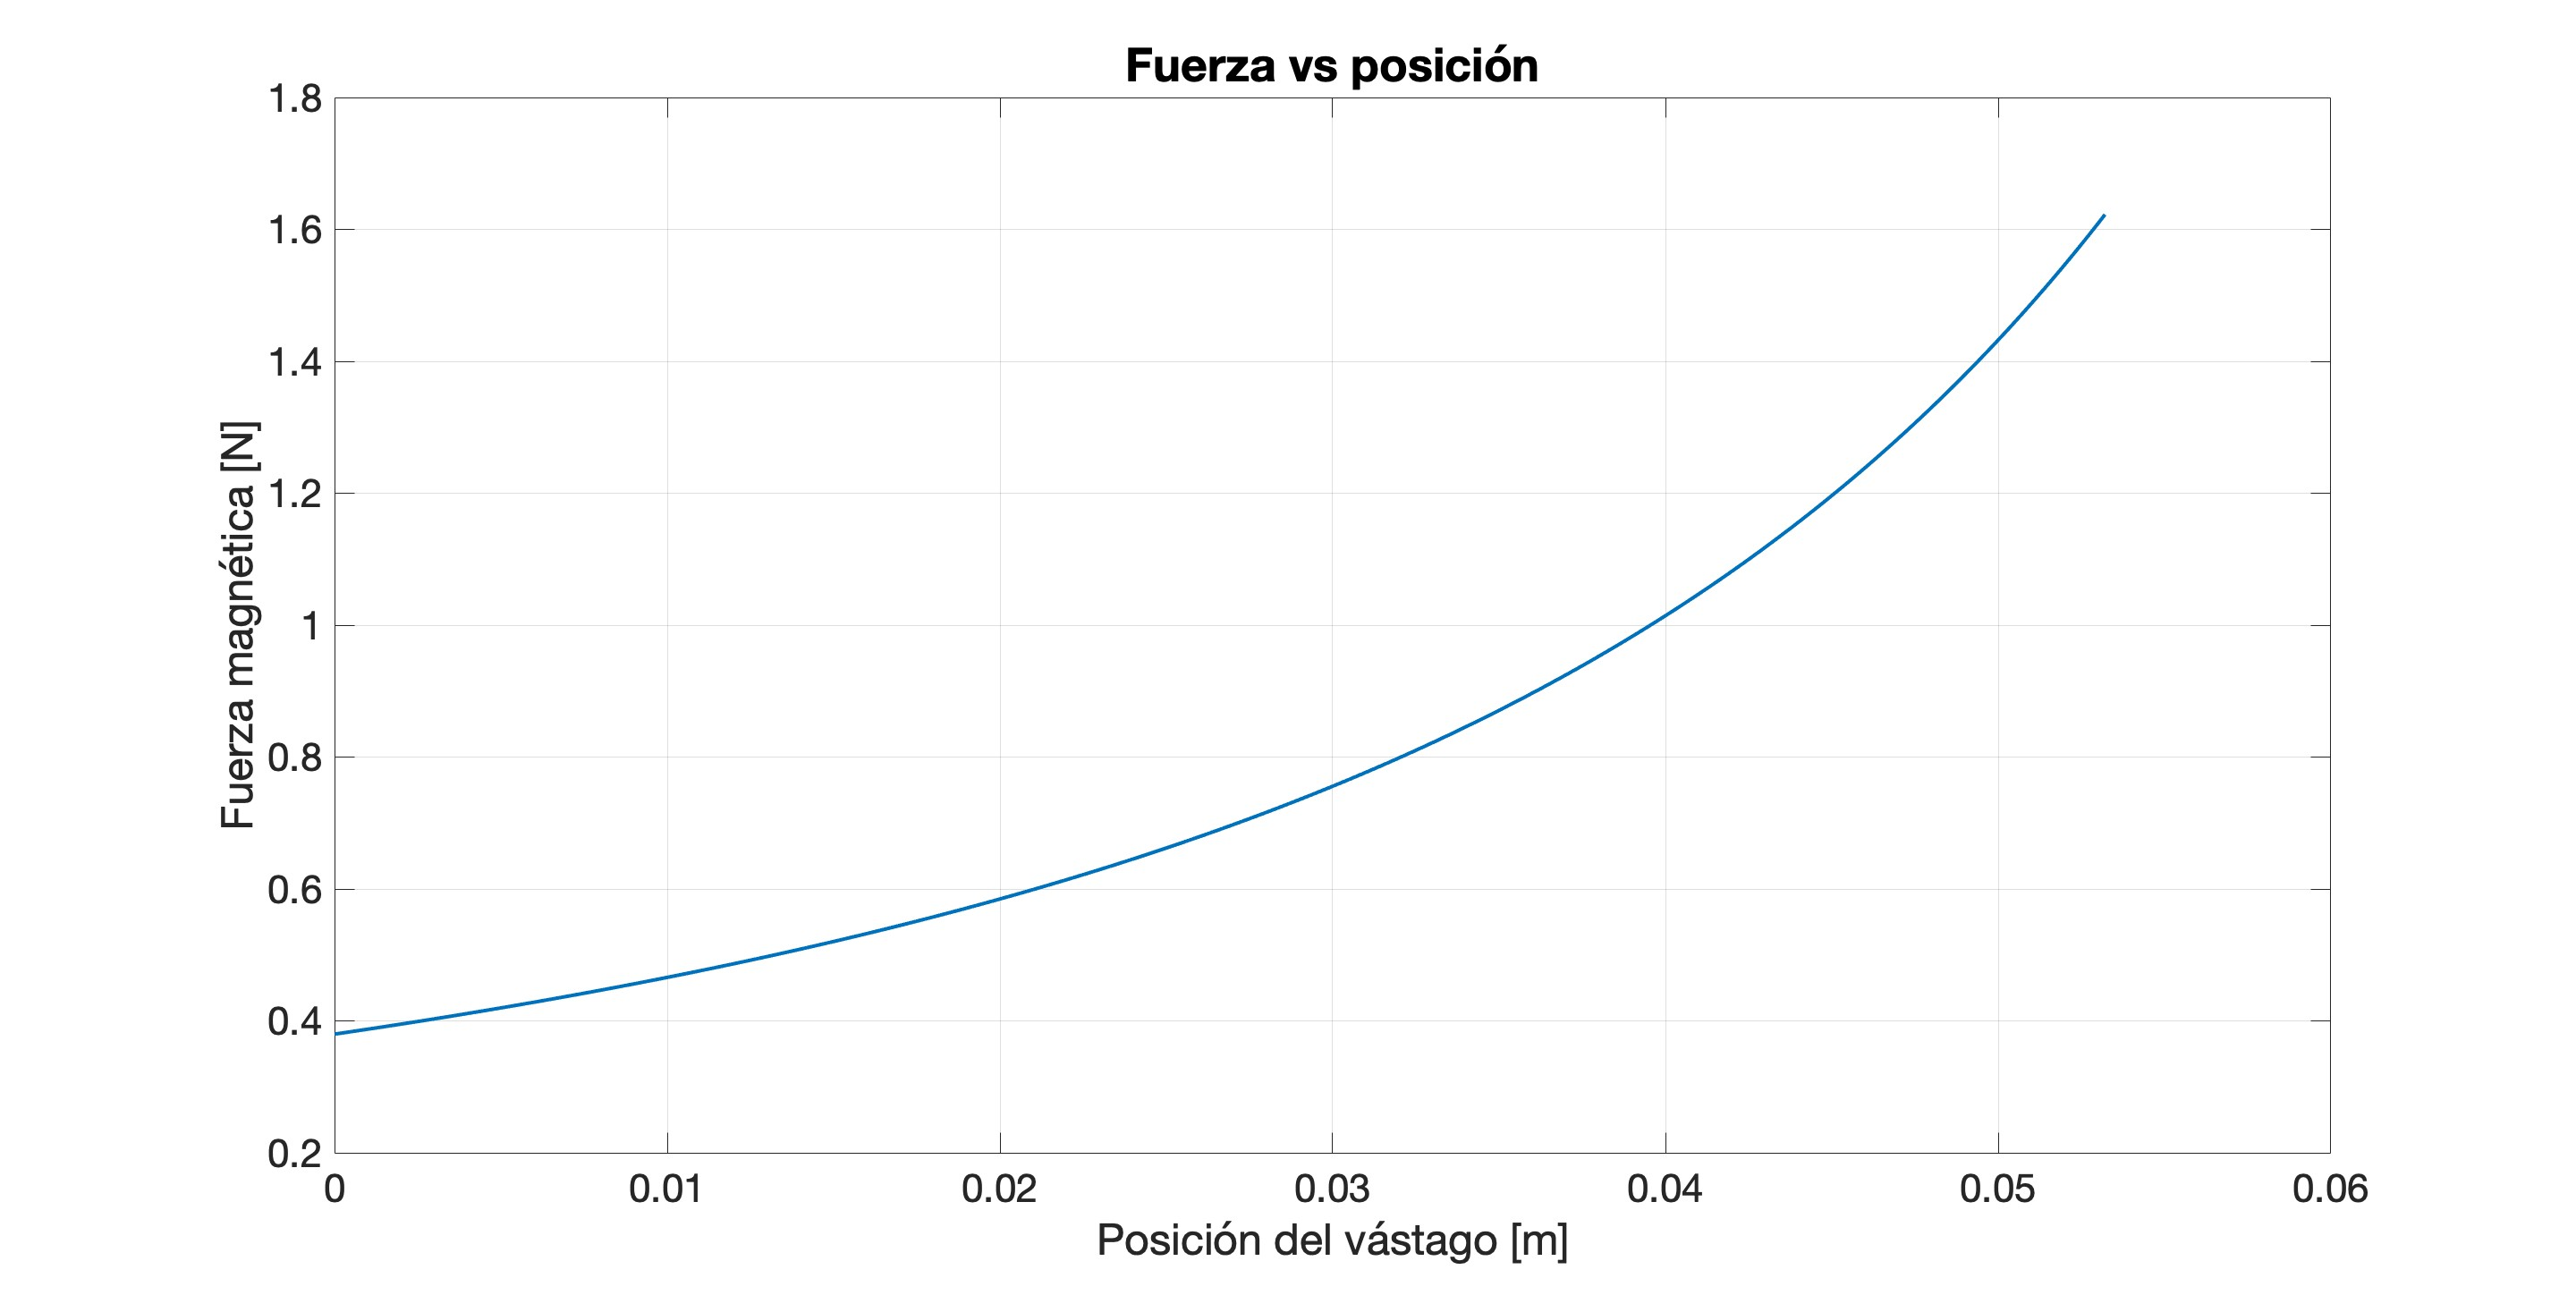
\includegraphics[width=\linewidth]{FigurasMemoria/calcFsetupBase.jpg}
    \caption{Fuerza en función de la posición del vástago respecto a la bobina.}
    \label{fig:calcFsetupBase} %Para referenciar -> \ref{fig:figNum}
\end{figure}

Estas figuras serán discutidas en el apartado de análisis de resultados (\ref{sec:resultados}).

\subsubsection*{Prueba inicial}

Antes de continuar con el desarrollo, se ha realizado una prueba con un dinamómetro sobre la bobina de prueba especificada anteriormente, para verificar los resultados de la figura \ref{fig:calcFsetupBase} y poder continuar con las simulaciones y prototipo con una referencia. Se ha obtenido el siguiente resultado:

\begin{figure}[H]
    \centering
    
\includegraphics[width=9cm]{FigurasMemoria/dinamometro.jpeg}
    \caption{Dato experimental de fuerza con la bobina alimentada.}
    \label{fig:dinamometro} %Para referenciar -> \ref{fig:figNum}
\end{figure}

\[F_{barra}=2.4~N~\forall I_{cc}=3.5~A\]